\section{The Magnus induction}\label{mag:section}

We now apply Theorem~\ref{ann:combination} to one-relator groups.
The geometric form of the Magnus construction gives an HNN extension
whose vertex group has smaller complexity and whose edge groups are
simultaneous Magnus subgroups.  The induction will establish
hyperbolicity.  At each stage, Linton's theorem on Magnus subgroups
of hyperbolic one-relator groups supplies the quasiconvexity needed
by the combination theorem.

\subsection{Graph presentations and Magnus subgroups}

Let $\Gamma$ be a finite connected graph, and let
$\lambda\colon S^1\to\Gamma$ be a nontrivial immersed combinatorial
circuit.  Write
\[
 X=\Gamma\cup_\lambda D^2,
 \qquad S_\lambda=\lambda(S^1).
\]
We call a connected subgraph $\Delta\subset\Gamma$ a
\emph{Magnus subgraph} if $S_\lambda\not\subset\Delta$; equivalently,
$\Delta$ omits an edge traversed by $\lambda$.
The following observation relates this definition to the usual
generator-subset definition.

\begin{lemma}\label{mag:graph-magnus}
Let $X=\Gamma\cup_\lambda D^2$ be as above, and let
$\Delta\subset\Gamma$ be a Magnus subgraph.  There is a free basis
$\Sigma$ of $\pi_1\Gamma$ in which $\pi_1\Delta$ is generated by a
subset of $\Sigma$ omitting a letter occurring in the cyclically
reduced relator.  Consequently, $\pi_1\Delta\to\pi_1X$ is injective.
Changing the path to the basepoint only conjugates its image.
\end{lemma}

\begin{proof}
Choose a spanning tree $T_\Delta$ of $\Delta$ and extend it to a
spanning tree $T$ of $\Gamma$.  The edges outside $T$ give the basis
$\Sigma$, and those in $\Delta\setminus T_\Delta$ give the indicated
subset.  Collapsing $T$ turns $\lambda$ into a nonempty cyclically
reduced word: cancellation between consecutive non-tree edges,
including at the cyclic join, would require a closed tree segment
between an edge and its inverse.  A nonempty such segment cannot
be reduced in a tree, while an empty segment would already be
backtracking in $\lambda$.

Suppose that this word used only the letters from $\Delta$.
Between consecutive non-tree edges of $\lambda$, its tree segment
is the unique tree path between vertices of $\Delta$.
That path lies in $T_\Delta$.  Every segment of $\lambda$ would
therefore lie in $\Delta$, contrary to the hypothesis.
The omitted-letter condition follows.  The injection is the
Freiheitssatz; see \cite[Theorem~1]{McCoolSchupp1973}.
\end{proof}

We use Linton's theorem in the following form:
every Magnus subgroup of a hyperbolic one-relator group is
quasiconvex \cite[Theorem~4.7]{LintonHyperbolic2026}.
Together with Lemma~\ref{mag:graph-magnus}, it applies to connected
Magnus subgraphs of any graph presentation whose group has already
been shown to be hyperbolic.

\subsection{A finite domain in a cyclic cover}

We use the geometric Magnus construction developed in
\cite[Section~4]{LintonHierarchies2025}, giving the domain and
complexity arguments in the form needed here.  The construction
finds a finite part of a cyclic cover whose adjacent overlaps
will supply the two Magnus subgroups in an HNN splitting.

For a graph of rank at least two, choose an epimorphism
\[
 \phi\colon\pi_1\Gamma\longrightarrow\mathbb Z
 \quad\text{with}\quad\phi([\lambda])=0.
\]
Such a map exists: the abelianized relator imposes at most one
equation on the integral characters of a free abelian group of
rank at least two, and dividing a nonzero solution by the gcd of
its coefficients makes it surjective.
Let $p\colon\widetilde\Gamma\to\Gamma$ be the corresponding
connected cyclic cover, with deck transformation $\tau$ of height
one.  A \emph{domain} will mean a finite connected subgraph
$D\subset\widetilde\Gamma$ such that the occurrences of every
base vertex and every base open edge form a nonempty interval of
translates.  Thus, after choosing any lift $\widetilde c$ of a base cell $c$, the
set
\[
 \{n\in\mathbb Z:\tau^n\widetilde c\subset D\}
\]
is a nonempty finite interval.  In particular, the translates of
a domain cover $\widetilde\Gamma$.  The following tree-overlap
construction is the graph case of
\cite[Lemma~4.7]{LintonHierarchies2025}.

\begin{lemma}\label{mag:tree-domain}
Every connected cyclic cover of a finite connected graph has a
domain $D$ for which $D\cap\tau D$ is a nonempty tree.
\end{lemma}

\begin{proof}
Choose a spanning tree downstairs.  We may then index the lifted
vertices by $(v,n)$ so that tree edges preserve $n$, while each
oriented non-tree edge has an integral increment $d_e$.
These increments generate $\mathbb Z$.
Let $D_N$ be the subgraph induced by all vertex types at levels
$[-N,N]$.  For sufficiently large $N$, every base edge occurs and
its occurrences form an interval.

We verify connectivity, including near the boundary of the
interval.  Choose a word in the signed increments whose sum is
$1$, and bound the absolute values of all its partial sums by
$L$.  Its translates connect consecutive levels whenever those
levels are sufficiently far from the ends of $[-N,N]$; the lifted
spanning trees connect the different vertex types at each level.
Choose also a nonzero increment, with absolute value $a$.
From a level near the lower boundary, repeated steps of size
$a$ in the positive direction reach the interior, and from the
upper boundary repeated negative steps do the same.  For
$N>L+a$, these steps remain in the interval and reach the
connected interior.  Thus $D_N$ is connected.  The identical
argument applies to the interval $[-N+1,N]$, whose induced
subgraph is $D_N\cap\tau D_N$.

Among domains with connected nonempty adjacent overlap, choose
$D$ with the fewest edges.  If $D\cap\tau D$ contains a circuit,
choose a simple one and translate it upward as long as it remains
in $D$.  Every position reached remains in $D\cap\tau D$,
because its preceding translate lies in $D$.
At the last position, some edge $e$ of the circuit has
$\tau e\notin D$.  Since $e\in D\cap\tau D$, its preceding
translate $\tau^{-1}e$ does lie in $D$.
Delete the open edge $e$, retaining its endpoints.
It was the highest occurrence of its base edge, so all occurrence
intervals remain nonempty intervals.  Moreover,
\[
 (D\setminus e)\cap\tau(D\setminus e)
   =(D\cap\tau D)\setminus e,
\]
because $\tau e\notin D$.
Both graphs remain connected: the deleted edge lies on a circuit
in their common overlap.  This contradicts minimality.
The overlap is therefore a nonempty tree.
\end{proof}

We next enlarge or modify such a domain to contain one lifted
relator.  Its two overlaps will become the edge groups of the
splitting.  The construction also accounts for strict decrease
of the complexity
\begin{equation}\label{mag:complexity}
 c(\Gamma,\lambda)=
 \bigl(|\lambda|-|V(S_\lambda)|,
             \operatorname{rank}\pi_1\Gamma\bigr),
\end{equation}
ordered lexicographically.  Here $|\lambda|$ counts edge
traversals, with multiplicity.  The first coordinate is
nonnegative, since an immersed circuit visits at most one new
vertex per edge traversal.  Up to an additive constant in its
second coordinate, this is the non-power form of the complexity
used for one-relator hierarchies
\cite[Section~4.3]{LintonHierarchies2025}.

\begin{lemma}\label{mag:splitting}
Suppose $\operatorname{rank}\pi_1\Gamma\geq2$ and that $\lambda$
represents a non-power in $\pi_1\Gamma$.
There are a domain $U\subset\widetilde\Gamma$ and a closed lift
$\widetilde\lambda\colon S^1\to U$ with the following properties.
Set
\[
 U_-=U\cap\tau^{-1}U,\qquad U_+=U\cap\tau U,
 \qquad Z=U\cup_{\widetilde\lambda}D^2.
\]
Both $U_-$ and $U_+$ are connected nonempty Magnus subgraphs of
$Z$.  Either both are trees, or $U_-\cap U_+$ is connected and
nonempty.  Their fundamental groups are simultaneous Magnus
subgroups in a presentation of $H=\pi_1Z$, and
\begin{equation}\label{mag:hnn}
 \pi_1X\cong\langle H,t\mid tAt^{-1}=B\rangle,
 \qquad A=\pi_1U_-,\quad B=\pi_1U_+,
\end{equation}
with edge isomorphism induced by $\tau$ and suitable basepoint
paths.  The vertex and edge groups inject, the lifted relator is
a non-power, and
\[
 c(U,\widetilde\lambda)<c(\Gamma,\lambda).
\]
\end{lemma}

\begin{proof}
We first construct $U$ and prove the complexity decrease, using
two cases according to the projection of the lifted support.
We then verify the HNN splitting and the simultaneous Magnus
bases for both constructions.  This is the domain method of
\cite[Propositions~4.9 and~4.11]{LintonHierarchies2025}.

\smallskip\noindent
\emph{Case 1: the lifted support does not project injectively on vertices.}
Take $D$ from
Lemma~\ref{mag:tree-domain} and let
\[
 U=\bigcup_{i=0}^{m}\tau^iD,
\]
where $m\geq0$ is the least integer for which this union contains
some closed lift $\widetilde\lambda$.
Such an integer exists: translate a fixed finite lifted circuit
far enough in the positive direction, and then take a sufficiently
long interval of translates of $D$.
The graph $U$ is connected and its cell occurrences are intervals.
Indeed, an occurrence interval $[a,b]$ in $D$ becomes $[a,b+m]$
in $U$.  Figure~\ref{mag:domain-intervals} shows how taking
adjacent overlaps trims the endpoints of this interval.

\begin{figure}[!hb]
\centering
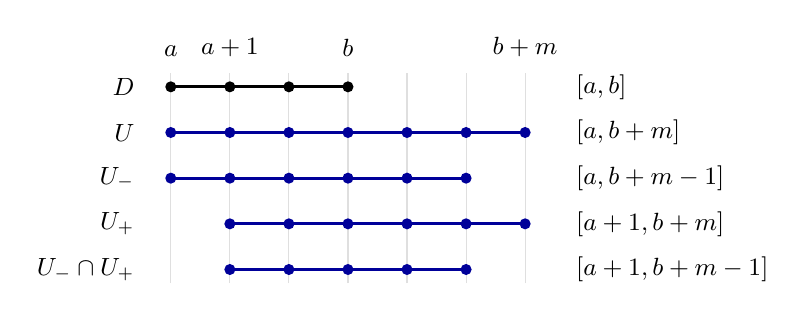
\begin{tikzpicture}[x=.75cm,y=.58cm,font=\small]
  \foreach \x in {0,...,6}
    \draw[gray!25] (\x,-.3)--(\x,4.3);
  \node[above] at (0,4.45) {$a$};
  \node[above] at (1,4.45) {$a+1$};
  \node[above] at (3,4.45) {$b$};
  \node[above] at (6,4.45) {$b+m$};
  \node[anchor=east] at (-.45,4) {$D$};
  \node[anchor=east] at (-.45,3) {$U$};
  \node[anchor=east] at (-.45,2) {$U_-$};
  \node[anchor=east] at (-.45,1) {$U_+$};
  \node[anchor=east] at (-.45,0) {$U_-\cap U_+$};
  \draw[very thick] (0,4)--(3,4);
  \draw[very thick,blue!60!black] (0,3)--(6,3);
  \draw[very thick,blue!60!black] (0,2)--(5,2);
  \draw[very thick,blue!60!black] (1,1)--(6,1);
  \draw[very thick,blue!60!black] (1,0)--(5,0);
  \foreach \x in {0,...,3} \fill (\x,4) circle (2pt);
  \foreach \x in {0,...,6} \fill[blue!60!black] (\x,3) circle (2pt);
  \foreach \x in {0,...,5} \fill[blue!60!black] (\x,2) circle (2pt);
  \foreach \x in {1,...,6} \fill[blue!60!black] (\x,1) circle (2pt);
  \foreach \x in {1,...,5} \fill[blue!60!black] (\x,0) circle (2pt);
  \node[anchor=west] at (6.7,4) {$[a,b]$};
  \node[anchor=west] at (6.7,3) {$[a,b+m]$};
  \node[anchor=west] at (6.7,2) {$[a,b+m-1]$};
  \node[anchor=west] at (6.7,1) {$[a+1,b+m]$};
  \node[anchor=west] at (6.7,0) {$[a+1,b+m-1]$};
\end{tikzpicture}
\caption{Occurrence intervals for one fixed base cell in Case~1,
illustrated with $b-a=m=3$.  Each point represents a translate of
that cell, not a copy of the domain $D$.  The formulas also apply
when $m=0$, with an interval empty if its lower endpoint exceeds
its upper endpoint.  In that case $U=D$, and the complete adjacent
overlap graphs are nonempty trees by Lemma~\ref{mag:tree-domain}.}
\label{mag:domain-intervals}
\end{figure}

If $m=0$, both adjacent overlaps are trees.  If $m\geq1$, the
interval calculation gives
\[
 U_- =\bigcup_{i=0}^{m-1}\tau^iD,
 \qquad
 U_+ =\bigcup_{i=1}^{m}\tau^iD.
\]
Minimality of $m$ shows that neither contains a closed lift of
$\lambda$.  Their intersection is
\[
 U_-\cap U_+=
 \begin{cases}
   D\cap\tau D,&m=1,\\
   \displaystyle\bigcup_{i=1}^{m-1}\tau^iD,&m\geq2.
 \end{cases}
\]
It is connected and nonempty.  In the case $m=0$, a tree cannot
contain the nontrivial immersed circuit, so the overlaps are
again Magnus subgraphs.
The lifted circuit has the same length as $\lambda$ and strictly
more support vertices.  Thus the first coordinate of
\eqref{mag:complexity} has decreased.

\smallskip\noindent
\emph{Case 2: the lifted support projects injectively on vertices.}
It then projects isomorphically onto $S_\lambda$:
two lifts of the same oriented edge cannot have the same initial
vertex.  The character therefore vanishes on
$\pi_1S_\lambda$, and every lift of this support is a copy of it.
Choose a spanning tree $T_S$ of $S_\lambda$ and extend it to a
spanning tree of $\Gamma$; in the resulting level coordinates
each support copy lies at one level.

Contract the support downstairs and every support copy upstairs.
This gives the connected cyclic cover of the quotient graph
$\Gamma/S_\lambda$ corresponding to the still-surjective
character.  Apply Lemma~\ref{mag:tree-domain} there.
Expand every occurrence of the contracted vertex in the resulting
domain by a copy of $T_S$.  At one chosen occurrence, add all the
remaining edges of $S_\lambda$.
Call the resulting graph $U$.  It is a connected domain:
the support-tree cells have the same occurrence interval as the
contracted vertex, and each added support edge has a singleton
occurrence interval.  The overlap $U\cap\tau U$ is a tree,
obtained by expanding vertices of a tree into trees; none of the
added support edges lies in it.  The full support at the chosen
occurrence contains a closed lift $\widetilde\lambda$.
Both overlaps are trees and hence Magnus subgraphs.

Here the first complexity coordinate is unchanged and the second
decreases.  To see this directly, for each base open cell its
number of occurrences in $U$ exceeds its number of occurrences
in $U\cap\tau U$ by one.  Counting vertices and edges gives
\[
 \chi(U)-\chi(U\cap\tau U)=\chi(\Gamma).
\]
Since the overlap is a tree, $\chi(U)=\chi(\Gamma)+1$, and hence
\[
 \operatorname{rank}\pi_1U
       =\operatorname{rank}\pi_1\Gamma-1.
\]

\smallskip\noindent
\emph{The HNN splitting.}
Both constructions now have the required overlaps and complexity
decrease.  We recover $X$ from the translates of $Z$, as in
\cite[Proposition~4.3]{LintonHierarchies2025}.  Since
$\phi([\lambda])=0$, the graph cover extends over the cells to
the cyclic cover $Y\to X$.  The translates $\tau^iZ$ cover $Y$,
and their two-cell interiors are distinct.
Form a line of disjoint copies of $Z$, joining each adjacent pair
by the cylinder on its intersection.  Denote this space by $W$;
collapsing these cylinders gives an equivariant map $W\to Y$.
For a finite interval of copies, the intersection of a newly
adjoined copy with the preceding union is precisely its adjacent
overlap.  Indeed, if a graph cell lies in the new copy and in an
earlier copy, its occurrence interval also puts it in the
immediately preceding copy.  Distinct copies have no common
two-cell interior, and cell boundaries consist of graph cells,
so this checks the entire intersection.
Van Kampen therefore shows inductively that the
cylinder-collapse map induces a fundamental-group isomorphism
over every finite interval.  Every loop and every homotopy uses
only finitely many copies, so $W\to Y$ induces an isomorphism on
fundamental groups as well.

Taking the quotient by translation gives a graph of spaces with
one vertex space $Z$ and one edge space, and a map
$W/\langle\tau\rangle\to X$.
The two covering exact sequences have quotient $\mathbb Z$;
the map is an isomorphism on their kernels and on this quotient.
It follows that it induces an isomorphism on fundamental groups.
The edge maps are injective by
Lemma~\ref{mag:graph-magnus}, because each overlap omits a
traversed relator edge.  Thus this graph of spaces gives the HNN
extension \eqref{mag:hnn}, and the normal form theorem gives
injection of $H$ into $\pi_1X$.

\smallskip\noindent
\emph{Simultaneous Magnus bases and the edge isomorphism.}
It remains to choose the two Magnus subsets simultaneously and
specify their basepoint paths.  If the overlap groups are trivial, this is
immediate.  Otherwise put $U_0=U_-\cap U_+$, which is connected
and nonempty by the construction.  Extend a spanning tree of
$U_0$ to spanning trees of $U_-$ and $U_+$.
Their intersection is exactly the chosen tree of $U_0$, so their
union is a tree.  Extend that union to a spanning tree of $U$.
With basepoint in $U_0$, the non-tree edges of the two overlaps
are then subsets of a single free basis of $\pi_1U$.
Their common letters freely generate $C=\pi_1U_0$, which is a
free factor in each side group.

To specify the stable letter in this nontrivial-edge case,
choose $x\in U_0$ and a path $q\subset U_+$ from $x$ to $\tau x$.
The latter vertex belongs to $U_+$ because $x\in U_-$.
Then $t=[p(q)]$ has height one, and the edge isomorphism sends a
loop $a$ in $U_-$ to $q\,(\tau a)\,q^{-1}$ in $U_+$.
Its projection is $tat^{-1}$, giving the specified isomorphism
in \eqref{mag:hnn}.
When the overlap groups are trivial, choose instead any
$x\in U_-$ and a path $q\subset U$ from $x$ to $\tau x$.
Again $t=[p(q)]$ has height one, and the edge relation is empty.
In either case, $q$ in the copy $Z$ closes in the quotient graph
of spaces by crossing the cylinder to the copy $\tau Z$ at
$\tau x$.  It crosses the quotient loop edge exactly once,
so it is a stable letter; collapsing the cylinder sends it to
$p(q)$.

Finally, $\pi_1U$ injects into $\pi_1\Gamma$, by inclusion into
the graph cover and its covering map.  If the lifted relator
were a proper power in $\pi_1U$, its image would be a proper
power in $\pi_1\Gamma$.  This proves the remaining assertion.
\end{proof}

\subsection{Hyperbolicity and the final reductions}

The preceding construction supplies the geometric input to the
combination theorem.  We now check its algebraic hypotheses.

\begin{proposition}\label{mag:nonpower-hyperbolicity}
Let $\Gamma$ be a finite connected graph, and let
$\lambda\colon S^1\to\Gamma$ be a nontrivial immersed circuit
representing a non-power in $\pi_1\Gamma$.
If $\pi_1(\Gamma\cup_\lambda D^2)$ is $BS$-free, then it is
word-hyperbolic.
\end{proposition}

\begin{proof}
We induct on the nonnegative lexicographic complexity
\eqref{mag:complexity}.  In graph rank one, the non-power relator
generates the infinite cyclic fundamental group, and the quotient
is trivial.  Rank zero cannot support the stipulated circuit.

In higher rank, apply Lemma~\ref{mag:splitting} to obtain
\[
 G=\langle H,t\mid tAt^{-1}=B\rangle.
\]
The vertex group $H$ embeds in $G$, and so is $BS$-free.
It has a non-power graph presentation of smaller complexity,
hence is hyperbolic by induction.  The one-relator torsion
theorem makes it torsion-free
\cite[Theorem~2]{McCoolSchupp1973}.
The side groups $A$ and $B$ are finitely generated free Magnus
subgroups of $H$; by
\cite[Theorem~4.7]{LintonHyperbolic2026}, they are quasiconvex in
$H$.

Use the simultaneous bases from Lemma~\ref{mag:splitting}.
Collins's conjugate-intersection theorem
\cite[Theorem~2]{Collins2008Conjugates}, which permits equal
Magnus subgroups, says that for $M,N\in\{A,B\}$ and $g\in H$,
\[
 M\cap gNg^{-1}\text{ noncyclic}\quad\Longrightarrow\quad g\in MN.
\]
This is the first overlap hypothesis of
Theorem~\ref{ann:combination}.
Collins's direct-intersection theorem
\cite[Theorem~1]{Collins2008Conjugates} gives
\[
 I=A\cap B=C\quad\text{or}\quad I=C*\langle u\rangle,
\]
where $C$ is generated by the common basis letters and the
second expression is an internal free product with an infinite
cyclic group.  Thus $I$ and its transported copy $J=t^{-1}It$
are finitely generated.
If the edge group is nontrivial, the two Magnus subgraphs
$U_-,U_+$ have connected intersection by the construction.
Linton's strong-inertia lemma
\cite[Lemma~2.10]{LintonHierarchies2025} states that the
intersection of the fundamental groups of two such Magnus
subgraphs is strongly inert in either side group.
It follows that $I$ is strongly inert in $P=A$ and in $B$.
Isomorphisms preserve reduced ranks and the indexing double
cosets, so transporting the latter assertion through the edge
isomorphism makes $J$ strongly inert in $P$ as well.
These are precisely the two strong reduced-rank inertia
inequalities in Theorem~\ref{ann:combination}.
When the edge group is trivial, the same requirements hold
directly.

All hypotheses of Theorem~\ref{ann:combination} have now been
verified.  Its conclusion makes $G$ hyperbolic, completing the
induction.
\end{proof}

\begin{proof}[Proof of Theorem~\ref{thm:main}]
Freely and cyclically reduce the defining relator; conjugating or
inverting it does not change its normal closure.
If it becomes trivial, the group is a finitely generated free
group and is hyperbolic.

If the cyclically reduced relator is a proper power, write it as
$w^k$, where $w$ is a nontrivial cyclically reduced non-power and
$k\geq2$.  Newman's spelling theorem
\cite{Newman1968}, in the form
\cite[Theorem~4]{McCoolSchupp1973}, says that every nonempty
freely reduced null word contains a segment of a cyclic conjugate
of $w^{\pm k}$ of length greater than $(k-1)|w|$.
This is strictly more than half the relator length, including
when $k=2$.  Replacing that segment by the inverse complementary
segment strictly shortens the word and uses one defining
relation.  Repeating, with free reduction after each replacement,
fills a null word with at most its original length in relator
cells.  These shortening rules give a finite Dehn presentation
(and a linear isoperimetric inequality).  The group is therefore
word-hyperbolic
\cite[Theorem~III.$\Gamma$.2.6]{BridsonHaefliger1999}.

In the remaining case, realize the cyclically reduced non-power
relator as an immersed circuit in the basis rose.
Proposition~\ref{mag:nonpower-hyperbolicity} applies and proves
hyperbolicity under the stated exclusion of $BS(m,n)$ for all
nonzero integers $m,n$.
\end{proof}

\begin{proof}[Proof of Theorem~\ref{thm:magnus}]
Under its non-power graph-presentation hypotheses,
Proposition~\ref{mag:nonpower-hyperbolicity} makes the ambient
group hyperbolic.  For any connected subgraph omitting a
traversed edge, Lemma~\ref{mag:graph-magnus} identifies its
fundamental group with an injective Magnus subgroup in a
one-relator presentation.  Linton's theorem
\cite[Theorem~4.7]{LintonHyperbolic2026} makes that subgroup
quasiconvex.  Basepoint paths only conjugate it, so the assertion
holds for every choice of such paths.
\end{proof}
